
En niveaumængde beskriver mængden af alle de mulige vektorer $\vec{x}$, som i funktionen $f(\vec{x})$ giver en bestemt funktionsværdi $z$. 
\begin{defn}[Niveaumængde]
Lad $f(\vec{x})= \vec{c}^T\vec{x}$ være en objektfunktion, da kaldes
\begin{align*}
N_z = \{\vec{x} \in \mathds{R}^n \mid f(\vec{x}) = z, \, z \in \mathds{R}\}
\end{align*}
for en \textbf{niveaumængde}.
\end{defn}



For et minimeringsproblem er målet derved at finde den mindste værdi $z$ for hvilken der findes en vektor $\vec{x}$, så $f(\vec{x})=z$, og hvor $\vec{x}$ overholder alle problemets betingelser.

Den mulige mængde beskriver alle vektorer $\vec{x}$, som opfylder betingelserne. Derved er målet at finde den mindste mulige $z$, for hvilken der er en ikke-tom skæring mellem niveaumængden $N_z$ og den mulige mængde.

\begin{stn}
Lad $N_z$ betegne en niveaumængde for en funktion $f(\vec{x})=\vec{c}^T\vec{x}$, da er $\vec{c}$ ortogonal med enhver $\vec{d}= \vec{x}-\vec{y}$ for alle $\vec{x}, \vec{y} \in N_z$. 
\end{stn}

\begin{proof}
Tages prikproduktet af $\vec{d}$ og $\vec{c}$, fås
\begin{align*}
\vec{c}^T\vec{d}=\vec{c}^T(\vec{x}-\vec{y}) = \vec{c}^T\vec{x} -\vec{c}^T\vec{y} = z - z = 0,
\end{align*}
hvorfor $\vec{c}$ og $\vec{d}$ er ortogonale i følge Lemma \ref{lma:vinkelret}.
\end{proof}
Det følger derfor, at niveaumængdens værdi ændres i $\vec{c}$s retning. 
Vælges derfor en vektor $\vec{x}=k\vec{c}$, vil denne vektor være en del af en niveaumængde hvor $\vec{c}^T\vec{x}=k\Vert\vec{c}\Vert^2=z$. Ved at isolere for $k$ findes det, at $k=\frac{z}{\Vert\vec{c}\Vert^2}$ når $k\vec{c}$ er en del af niveaumængden.

%Da $k$ er direkte proportionel med $z$ kan den optimale værdi i et maksimeringsproblem findes hvor  en funktion af $z$, kan den optimale værdi i et maksimeringsproblem findes for den niveaukurve, hvor 

En optimal løsning kan derved findes i maksimeringsproblemer, ved at finde den største mulige $k\vec{c}$, hvor den tilsvarende niveaumængde skærer den mulige mængde. Altså, bliver afstanden mellem niveaumængden og origo større jo større $z$ er, da $z$ er direkte proportionel med $k$. Tilsvarende må det gælde modsat for minimeringsproblemer. 
Altså kan en niveaumængde vises geometrisk som en mængde, der er ortogonal på $\vec{c}$ og indeholder vektoren $k\vec{c}=\frac{z}{\Vert\vec{c}\Vert^2}\vec{c}$.

%
%Dette betyder derved at der ved grafisk at undersøge en mulig mængde vil være muligt for minimeringsproblemer af finde den optimale løsning der hvor en skæringen mellem niveaukurven og den mulige mængde er ikke-nul og hvor skæringen går igennem den vektor $\vec{c}k$ med mindst mulig $k$.
%dette fungerer tilsvarende med størst mulig $k$ for maksimeringsproblemer.

Denne teori er i Eksempel \ref{eks:maksprob3} anvendt til at finde punktet med den optimale værdi for et givet programmeringsproblem.

\begin{eks}[Optimal løsning fundet grafisk for maksimeringsproblem]
Niveaumængderne $46=\vec{c}^T \vec{x}$ og $25=\vec{c}^T \vec{x}$ er på Figur \ref{fig:maksprob3} indtegnet for programmeringsprogblemet fra Eksempel \ref{eks:maksprob2}.

	\begin{center}	
		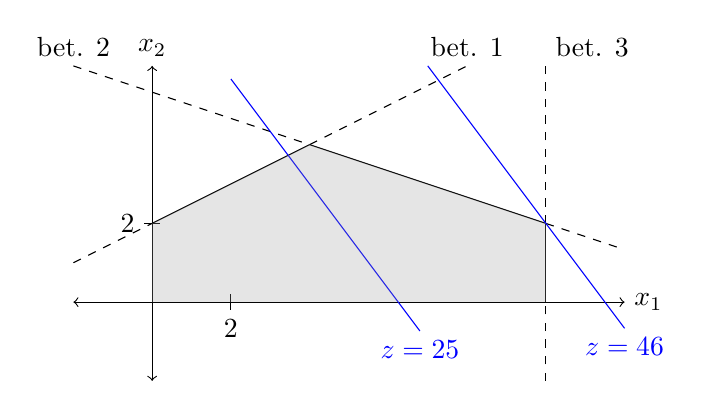
\begin{tikzpicture}
  %laver Grid. godt til når koordinater skal redigeres
  	%\draw[thin,gray!40] (-3,-1) grid (6,3); 
  %x-aksen
  	\draw[<->] (-1,0)--(6,0) node[right]{$x_1$}; 
  %y-aksen
  	\draw[<->] (0,-1)--(0,3) node[above]{$x_2$};
  	
  %akse-markeringer
  	%\node[left] (xakse) at (0,1) {2};
  	\draw[] (-0.1,1) -- (0.1,1) node[pos=0,left] {2};
  	\draw[] (1,-0.1) -- (1,0.1) node[pos=0,below] {2};
  	
  %ligning 1
	\draw[domain=-1:0,variable=\x,dashed] 	plot({\x},{0.5*\x+1});
	\draw[domain=0:2,variable=\x] 			plot({\x},{0.5*\x+1});
	\draw[domain=2:4,variable=\x,dashed] 	plot({\x},{0.5*\x+1}) node[above] {bet. 1};
	
  %ligning 2
  	\draw[domain=-1:2,variable=\x,dashed] 	plot({\x},{-(1/3)*\x+8/3}) node[above] at (-1,3) {bet. 2} ;
	\draw[domain=2:5,variable=\x] 			plot({\x},{-(1/3)*\x+8/3});
	\draw[domain=5:6,variable=\x,dashed] 	plot({\x},{-(1/3)*\x+8/3});
	

  %ligning 3
  	\draw[domain=-1:0,variable=\y,dashed] 	plot({5},{\y});
	\draw[domain=0:1,variable=\y] 			plot({5},{\y});
	\draw[domain=1:3,variable=\y,dashed] 	plot({5},{\y}) node[above right] {bet. 3};
	
  %niveaukurver
  	\draw[domain=3.5:6,variable=\x,blue] plot({\x},{-(4/3)*\x+23/3}) node[below] {$z=46$};
  	\draw[domain=1:3.4,variable=\x,blue] plot({\x},{-(4/3)*\x+25/6}) node[below] {$z=25$};
  	
  %c-vektor
  	%\draw[->,thick,red] (0,0) -- (2,1.5);

  %løsningsmængden skraveret
	\fill[gray!80,nearly transparent] (0,0) -- (0,1) -- (2,2) -- (5,1) --(5,0) --  cycle;
\end{tikzpicture}
		\captionof{figure}{Optimal løsning i den mulige mængde fundet som skæring med ligningen $z=46$.}
		\label{fig:maksprob3}
	\end{center}
	
På figuren ses det, at den største funktionsværdi $z=46$ findes i skæringen mellem bibetingelse 2 og 3.
Ved at løse bibetingelse 2 og 3 som 2 ligninger med 2 ubekendte findes det, at den optimale løsning er $\vec{x}=\rvect{10 & 2}^T.$
Øges $k$ på figuren, vil den tilsvarende niveaumængde og den mulige mængde ikke længere have en ikke-nul skæring. 

\label{eks:maksprob3}
\end{eks}





